% !TEX TS-program = pdflatex
% !TEX encoding = UTF-8 Unicode

% This is a simple template for a LaTeX document using the "article" class.
% See "book", "report", "letter" for other types of document.

\documentclass[11pt]{article} % use larger type; default would be 10pt

\usepackage[utf8]{inputenc} % set input encoding (not needed with XeLaTeX)

%%% Examples of Article customizations
% These packages are optional, depending whether you want the features they provide.
% See the LaTeX Companion or other references for full information.

%%% PAGE DIMENSIONS
\usepackage{geometry} % to change the page dimensions
\geometry{a4paper} % or letterpaper (US) or a5paper or....
% \geometry{margin=2in} % for example, change the margins to 2 inches all round
% \geometry{landscape} % set up the page for landscape
%   read geometry.pdf for detailed page layout information

\usepackage{graphicx} % support the \includegraphics command and options

% \usepackage[parfill]{parskip} % Activate to begin paragraphs with an empty line rather than an indent

%%% PACKAGES
\usepackage{booktabs} % for much better looking tables
\usepackage{array} % for better arrays (eg matrices) in maths
\usepackage{paralist} % very flexible & customisable lists (eg. enumerate/itemize, etc.)
\usepackage{verbatim} % adds environment for commenting out blocks of text & for better verbatim
\usepackage{subfig} % make it possible to include more than one captioned figure/table in a single float
% These packages are all incorporated in the memoir class to one degree or another...

%%% HEADERS & FOOTERS
\usepackage{fancyhdr} % This should be set AFTER setting up the page geometry
\pagestyle{fancy} % options: empty , plain , fancy
\renewcommand{\headrulewidth}{0pt} % customise the layout...
\lhead{}\chead{}\rhead{}
\lfoot{}\cfoot{\thepage}\rfoot{}

%%% SECTION TITLE APPEARANCE
\usepackage{sectsty}
\allsectionsfont{\sffamily\mdseries\upshape} % (See the fntguide.pdf for font help)
% (This matches ConTeXt defaults)

%%% ToC (table of contents) APPEARANCE
\usepackage[nottoc,notlof,notlot]{tocbibind} % Put the bibliography in the ToC
\usepackage[titles,subfigure]{tocloft} % Alter the style of the Table of Contents
\renewcommand{\cftsecfont}{\rmfamily\mdseries\upshape}
\renewcommand{\cftsecpagefont}{\rmfamily\mdseries\upshape} % No bold!

%%% END Article customizations

%%% The "real" document content comes below...

\title{CS338 HW1}
\author{Brock Ellefson}
%\date{} % Activate to display a given date or no date (if empty),
         % otherwise the current date is printed 

\begin{document}
\maketitle
\section{}
\subsection{State Diagrams of DFA}
%(1.1) Problem 1.6.c, 1.6.f (page 84� all the questions with only numbers given are
%referred to the 3rd edition of the textbook).


	\begin{figure}[h]
		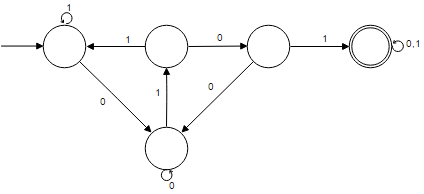
\includegraphics[scale = .75]{dfa1.png}
  		\caption{ $\lbrace$w$\mid$w contains the substring 0101 $($i.e., w = x0101y for some x and y$)$$\rbrace$}
  		\label{fig:dfa1}
	\end{figure}


	\begin{figure}[h]
  		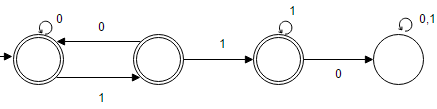
\includegraphics[scale = .75]{dfa2.png}
  		\caption{ $\lbrace$w$\mid$w doesn't contain the substring 110$\rbrace$}
  		\label{fig:dfa2}
	\end{figure}



\subsection{State Diagrams of NFA}
%(1.2) Problem 1.7.b, 1.7.c (page 84)

	\begin{figure}[h]
		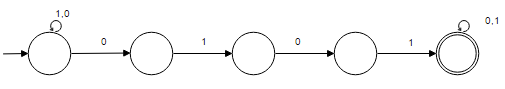
\includegraphics[scale = .75]{dfa3.png}
 		\caption{ $\{$w$\mid$w contains the substring 0101 $($i.e., w = x0101y for some x and y$)$$\}$}
  		\label{fig:dfa3}
	\end{figure}


	\begin{figure}[h]
  		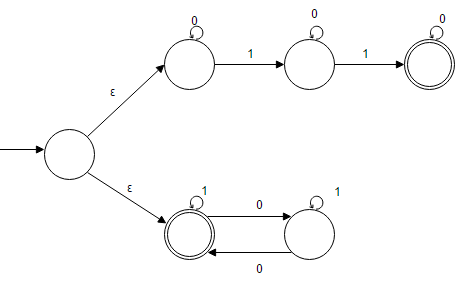
\includegraphics[scale = .75]{dfa42.png}
  		\caption{ $\{$w$\mid$w has either an even amount of 0's or exactly 2 1's$\}$}
  		\label{fig:dfa4}  
	\end{figure} 



\section{NFA to DFA}
%Problem 1.16.a, 1.16.b (page 86).

	\begin{figure}[h]
  		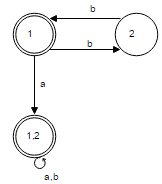
\includegraphics[scale = .75]{dfa5.png}
  		\caption{ 1.16 part a}
  		\label{fig:dfa5}  
	\end{figure} 
	
	\begin{figure}[h!]
  		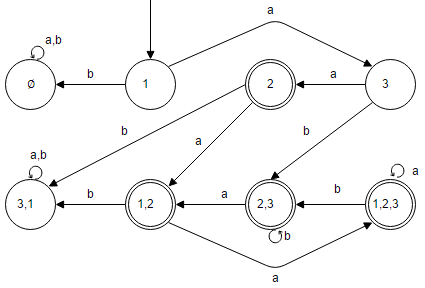
\includegraphics[scale = .7]{dfa6.png}
  		\caption{ 1.16 part b}
  		\label{fig:dfa6}  
	\end{figure} 	


\section{Regular Expression to NFA}
%Problem 1.19.a, 1.19.b (page 86).

	\begin{figure}[h!]
  		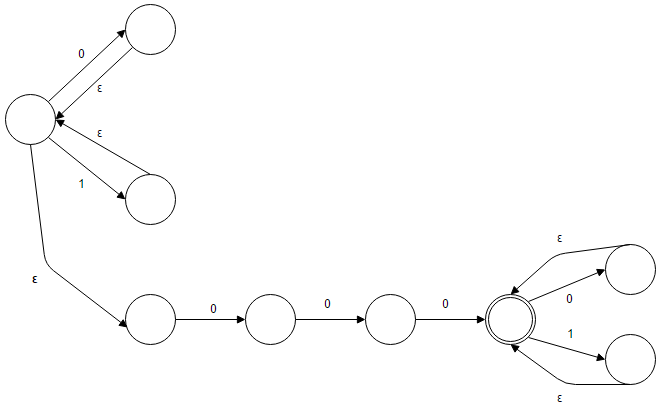
\includegraphics[scale = .75]{dfa7.png}
  		\caption{ $($0 U 1$)$$\ast$ 000 $($0 U 1$)$$\ast$}
  		\label{fig:dfa7}  
	\end{figure} 

	\begin{figure}[h!]
  		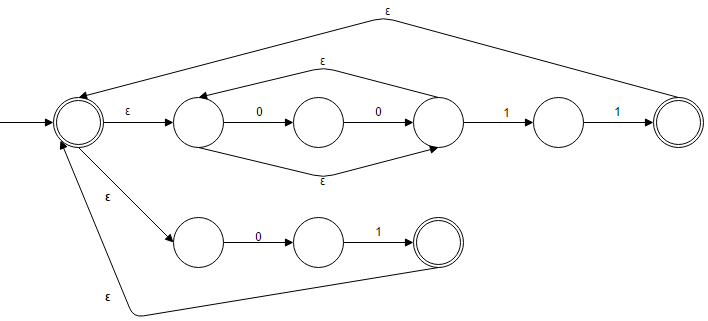
\includegraphics[scale = .75]{dfa8.png}
  		\caption{$($$($$($00$)$$\ast$$($11$)$$)$ U 01$)$$\ast$}
  		\label{fig:dfa8}  
	\end{figure} 
\newpage
\section{Finite Automata to Regular Expression}
%Problem 1.21a 
(a$^{\ast}$ba$^{\ast}$) U (a$^{\ast}$ba$^{\ast}$b)$^{\ast}$a$^{\ast}$ba$^{\ast}$

\section{Pumping Lemma}
\subsection{A = $\{$a$^{n}$$^{3}$$\mid$n$\geq$0$\}$}
Assume that A is a regular language. S = a$^{p}$$^{3}$\\
By the pumping lemma, S can be decomposed into xyz such that\\
 xy$^{i}$z $\in$ A \\
 $\mid$y$\mid$ $>$ 0 \\
 $\mid$xy$\mid$ $\leq$ P\\
As  xy$^{i}$z $\in$ A , y can only contains 1 'a' per pump\\
So, if we pump 2 times (i = 2),\\
xyz:\\
00000000\\
xyyz:\\
000000000\\
Then there will be 9 'a's after the second pump. This is not in the language.\\
This contradicts the pumping lemma\\
Therefore B is not a regular language.

\subsection{B = $\{$0$^{n}$1$^{m}$0$^{n}$$\mid$m,n$\geq$0$\}$}

Assume that B is a regular language. S = 0$^{p}$10$^{p}$\\
By the pumping lemma, S can be decomposed into xyz such that\\
 xy$^{i}$z $\in$ A \\
 $\mid$y$\mid$ $>$ 0 \\
 $\mid$xy$\mid$ $\leq$ P\\
 \\
As $\mid$xy$\mid$ $\leq$ P, y can only contains k $>$ 0 amount of 0's.\\
So, if we pump 0 times (i = 0),\\
xy$^{0}$z\\
Then there will be 0$^{p-k}$ on the first set of 0's and 0$^{p}$ on the second set of 0's\\
This contradicts the pumping lemma\\
Therefore B is not a regular language.
\end{document}
